%!TEX program = xelatex
\documentclass[cn,black,11pt,normal]{elegantnote}
\usepackage{float}
\usepackage{hyperref}
\usepackage{amsmath}
\usepackage{amsfonts}
\usepackage{amssymb}
\usepackage{siunitx}[=v2]
\usepackage{fancyhdr}
\usepackage{newtxtext}
\usepackage{algorithm}
\usepackage{algorithmic}
\usepackage[final]{pdfpages}
\newcommand{\uct}[1]{\textsuperscript{\textsuperscript{\cite{#1}}}}
% \renewcommand{\tablename}{\textbf{Table}}
% \renewcommand{\figurename}{Figure.}
% \renewcommand{\refname}{References}
% \renewcommand{\contentsname}{Contents}
% \renewcommand{\versiontext}{Version: }
% \renewcommand{\updatetext}{Update: }
\PassOptionsToPackage{no-math}{fontspec}
\lstset{basicstyle=\footnotesize\ttfamily\color[RGB]{50,0,130},numbers=none,frame=trBL}

\sisetup{mode=text}
\sisetup{range-phrase = \text{ \textasciitilde }}
\pagestyle{fancy}
\fancyhead[L]{School of Software Engineering, Tongji University}
\fancyhead[R]{Compiler Project}
\renewcommand{\headrulewidth}{1pt}

\title{编译原理优化部分\\规划草稿}
\author{猫}
\institute{School of Software Engineering, Tongji University}
\version{0.01}
\date{\today}

\begin{document}

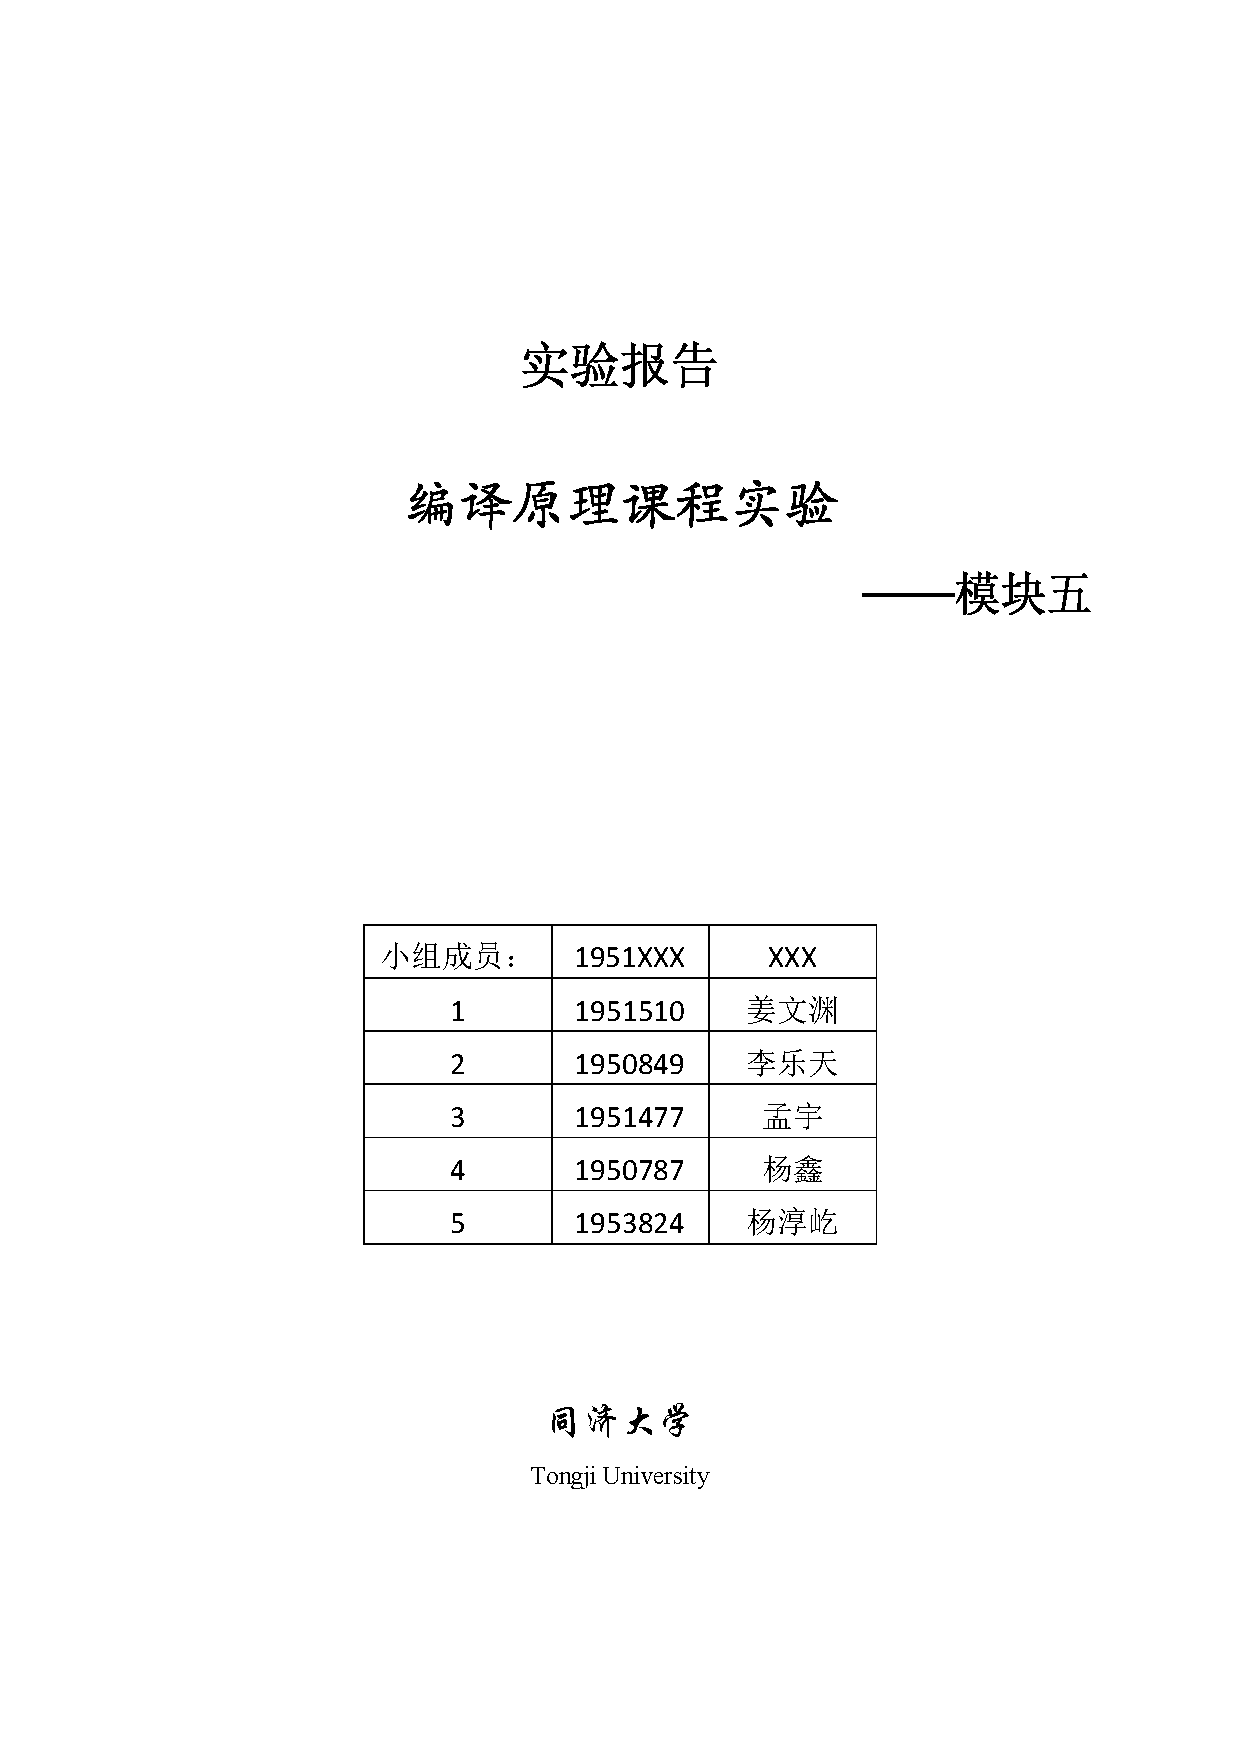
\includepdf{image/Cover.pdf} 
\newpage

\tableofcontents

\section{实验简介}

本次实验中,我们完成了语法分析后产生的三地址代码的优化,主要包括以下内容:

\begin{itemize}
    \item 局部优化:
    \subitem 基本块的划分
    \subitem 基本块的优化
    \item 循环优化:
    \subitem 循环不变量的查找与处理
    \subitem 代码外提
    \subitem 归纳变量的查找与处理
    \subitem 强度削弱
\end{itemize}

\section{实验原理}

\subsection{优化过程概览}

代码的优化过程主要分为两部分,一部分是对于以基本块为基础的局部优化,一部分是对于程序中的循环过程的优化。

对于局部优化,首先要进行基本块的划分,根据划分好的基本块进行DAG构造,应用DAG重写回中间代码我们可以实现对其的优化。

对于循环优化,主要有代码外提,强度削弱和删除归纳变量。

代码外提需要找到程序中的不变运算,再对运算进行判别是否可以外提。

强度削弱是将程序中执行时间长的运算转换为运算时间短的运算。主要是针对和基本归纳变量有线性关系的归纳变量的赋值运算进行。对于下标变量地址计算来说,强度削弱实际上就是实现下标变量地址的递归计算。

归纳变量为一类有特殊性质的变量,对于其识别与处理时强度削弱的前提。

\subsection{本次实验中使用的三地址代码}

本次实验中支持的三地址代码主要有两类:赋值与四则运算、跳转控制语句。

赋值与四则运算的语句格式如下所示:
\begin{lstlisting}
a = T_1
A [ i ] = T_1
T_1 = A [ i ]
T_1 = T_2 + T_3
T_1 = T_2 - T_3
T_1 = T_2 * T_3
T_1 = T_2 / T_3
T_1 = T_2 % T_3
\end{lstlisting}

跳转控制语句的格式列举如下:
\begin{lstlisting}
!: 101 // force jump
? T_1 > a : 101 // condition jump
? T_1 < a : 101 
? T_1 == a : 101 
? T_1 >= a : 101 
? T_1 <= a : 101 
? T_1 != a : 101 
HALT
\end{lstlisting}


\section{分析与实现}

\subsection{从三地址代码切分基本块}

结合实验代码,介绍具体的实现流程,对重要代码块进行解释说明
基本块指程序中一顺序执行语句序列,其中只有一个入口和一个出口。入口就是其中第一个语句,出口就是其中最后一个语句。

实现算法:

1. 求出三地址代码程序中各个基本块的入口语句:

1) 程序第一个语句,或

2) 能由条件转移语句或无条件转移语句转移到的语句,或

3) 紧跟在条件转移语句后面的语句。

2. 对以上求出的每个入口语句,确定其所属的基本块。它是由该入口语句到下一入口语句(不包括该入口语句)或到一转移语句(包括该转移语句)或一停语句(包括该停语句)之间的语句序列组成的。
根据以上算法原理可以轻松实现,具体的代码详见项目的GitHub库中的\url{https://github.com/42034301-5/OptimizerUtils/blob/main/split.py},这里受限于篇幅就不进行列出了。

\subsection{活跃变量的查找}

对于变量$x$和程序点$p$,如果在流图中沿着从$p$开始的某条路径会引用变量$x$在$p$点的值,则称变量$x$在点$p$是活跃(live)的,否则称变量$x$在点$p$不活跃(dead)。

有再次定值(且定值与本身无关),则不活跃。

活跃变量用于删除无用赋值,如果x在点p的定值在基本块内所有后继点都不被引用,且x在基本块出口之后又是不活跃的,那么x在点p的定值就是无用的。

活跃变量查找方法:

逆向数据流问题:

\begin{equation*}
    \begin{aligned}
        \text{IN}[B] &= f(\text{OUT}[B])\\
        f(x) &= \text{use}_B \cup (x - \text{def}_B)
    \end{aligned}
\end{equation*}

其中:
$\text{use}_B$是在基本块B中定值,但在定值前在B中没有被引用的变量的集合;
$\text{def}_B$是在基本块B中被引用,但是在引用前在B中没有被定值的变量集合。

\begin{figure}[H]
    \centering
    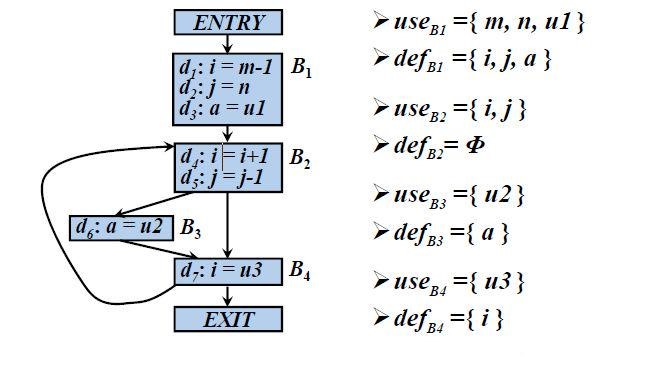
\includegraphics[width=0.8\linewidth]{image/activeV1.jpg}
    \caption{use与def集合的例子}
\end{figure}

构建各表达式use与def集合,如上图。
$\text{IN}[B]$:在基本块B的入口处的活跃变量集合;
$\text{OUT}[B]$:在基本块B的出口处的活跃变量集合。

使用下图所示的迭代算法,可以求得出各个基本块后的活跃变量的集合$\text{OUT}[B]$。

\begin{figure}[H]
    \centering
    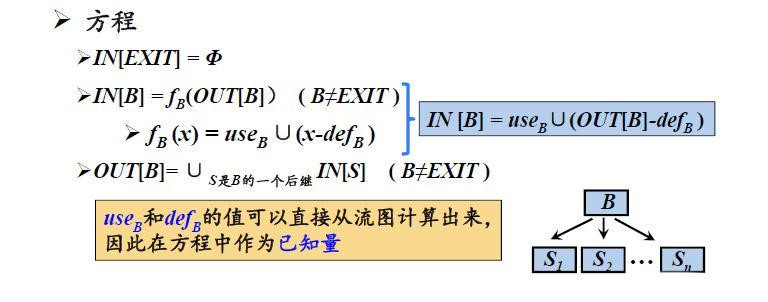
\includegraphics[width=0.8\linewidth]{image/activeV2.jpg}
    \caption{计算OUT集合的迭代算法}
\end{figure}

具体的代码详见项目的GitHub库中的\url{https://github.com/42034301-5/OptimizerUtils/blob/main/split.py}。

\subsection{自然循环查找}

自然循环是一种适合于优化的循环,满足以下性质:

1. 有唯一的入口结点,称为首结点(header)。首结点支配循环中的所有结点,否则,它就不会成为循环的唯一入口;

2. 循环中至少有一条返回首结点的路径,否则,控制就不可能从“循环”中直接回到循环头,也就无法构成循环。

\paragraph{识别方法:}
给定一个回边$n\rightarrow d$,该回边的自然循环为:$d$,以及所有可以不经过$d$而到达$n$的结点。$d$为该循环的首结点。如下图所示。

\begin{figure}[H]
    \centering
    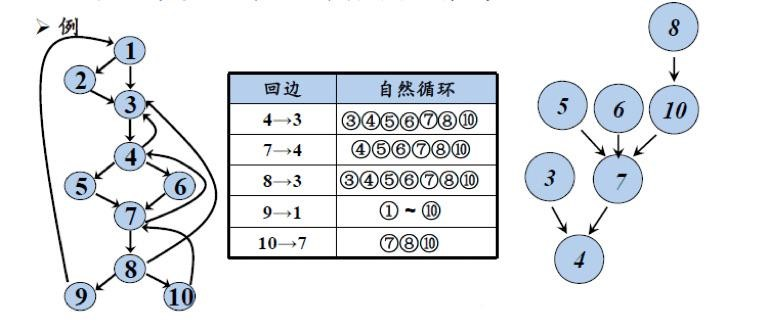
\includegraphics[width=0.8\linewidth]{image/findloop1.jpg}
    \caption{自然循环的例子}
\end{figure}

使用下图中的算法即可寻找出给定流图中的自然循环。

\begin{figure}[H]
    \centering
    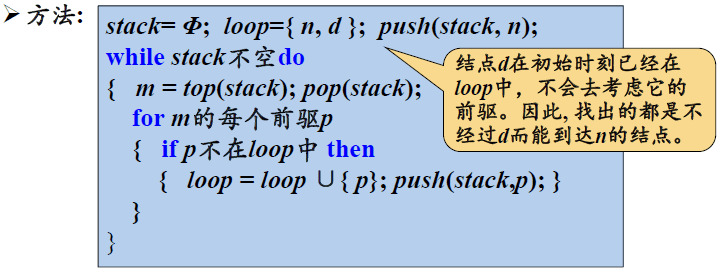
\includegraphics[width=0.8\linewidth]{image/findloop2.png}
    \caption{查找自然循环的算法}
\end{figure}

具体的代码详见项目的GitHub库中的\url{https://github.com/42034301-5/OptimizerUtils/blob/main/findloop.py}。

\subsection{基本块内优化}

\paragraph{DAG(有向无环图)的构造:}
基本块中的每个语句 s 都对应一个内部结点 N。
结点 N 的标号是 s 中的运算符;同时还有一个定值变量表被关联到 N ,表示 s 是在此基本块内最晚对表中变量进行定值的语
句。
N 的子结点是基本块中在 s 之前、最后一个对 s 所使用的运算分量进行定值的语句对应的结点。如果 s 的某个运算分量在基本块内没有在 s 之前被定值,则这个运算分量对应的子结点就是代表该运算分量初始值的叶结点。所有的字面常量都是叶子结点。在为语句 x = y + z 构造结点 N 的时候,如果 x 已经在某结点 M 的定值变量表中,则从 M 的定值变量表中删除变量 x。对于形如 x = y + z 的三地址指令,如果已经有一个结点表示 y + z ,就不往 DAG 中增加新的结点,而是给已经存在的结点附加定值变量。

构造完成示例如下图所示:

\begin{figure}[H]
    \centering
    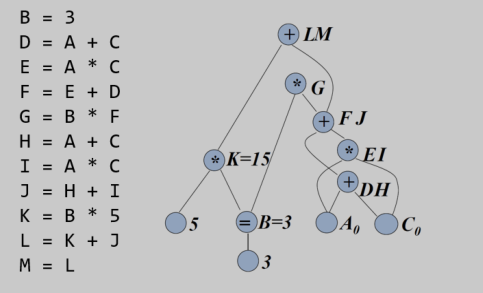
\includegraphics[width=0.8\linewidth]{image/dagopt1.png}
    \caption{DAG(有向无环图)的构造示例}
\end{figure}

\paragraph{从DAG生成三地址代码:} 从DAG生成优化后的代码需要在不产生无意义赋值的前提下以图结点的逆拓扑序生成,以确保代码之间的依赖关系正确。从所有根结点开始进行深度优先搜索并自下而上生成代码即可。此外,基本块内可能存在先引用外部变量再对其进行定值,以及对同一数组的多次读写操作,所以对DAG上互相没有依赖关系的结点也必须确保生成顺序正确,因此在DFS结点出栈生成代码前进行了额外的判断。


具体的代码详见项目的GitHub库中的\url{https://github.com/42034301-5/BlockOptimization}。

\subsection{从基本块生成三地址代码}

在还原的过程中只需要还原活跃变量。

通过流图中基本块的前驱与后继的关系,深度优先遍历基本块构成的流图,根据基本块内的代码行数预先分配需要填入代码的位置,逐行填入三地址代码。根据流图上边的关系填入跳转语句。最后删去多余的跳转语句即可。

具体的代码详见项目的GitHub库中的\url{https://github.com/42034301-5/OptimizerUtils/blob/main/blk2tri.py}。

\subsection{循环不变量的查找}

循环不变量即循环过程中数值保持不变的性质的量。

根据基本块中的变量定值信息,找出循环运算过程中的不变量,将等号右边均为循环不变量的式子标记为循环不变运算,同时将该式子左边的数也标记为循环不变量。按照顺序反复遍历基本块中的代码,直到不再发生变化即完成查找。


具体的代码详见项目的GitHub库中的\url{https://github.com/42034301-5/OptimizerUtils/blob/main/invariantOperationOfLoop.py}。

\subsection{代码外提}

找到循环不变运算以后,检查其中的每个式子:如果它所在的基本块是循环出口的必经节点,并且该式子定值的变量在其他基本块未定值,其他基本块对该变量的引用点一定会经过该式子,那么它可以外提;或者这个式子不是必经节点,但是它定值的变量离开该循环后不再活跃,并且它在其他基本块未定值,其他基本块对它的引用点一定会经过该基本块,那么这个式子也可以外提。

代码外提基本步骤:

\begin{enumerate}
    \item 求出L的所有不变运算
    \item 对每个不变运算s: \lstinline{A = B op C} 或 \lstinline{A = op B}  或 \lstinline{A = B}检查是否满足条件(1)或(2)。
        \subitem (1) i) s所在的结点是L所有出口结点的必经结点; ii) 且A在L中其他地方未再定值; iii) 且L中所有A的引用点只有s中的A的定值才能到达。
        \subitem (2) A在离开L后不再是活跃的,并且条件(1)的(ii)和(iii)成立。所谓A在离开L后不是活跃的是指,A在L的任何出口结点的后继结点入口处不是活跃的。
    \item 按步骤1所找出的不变运算的次序,依次把符合条件2的条件(1)或(2)的不变运算s外提到L的前置结点中。但是,如果s的运算对象(B或C)是在L中定值的,那么,只有当这些定值四元式都已外提到前置结点中时,才能把s也外提到前置结点中。
\end{enumerate}
根据上述步骤编写算法实现。

具体的代码详见项目的GitHub库中的\url{https://github.com/42034301-5/OptimizerUtils/blob/main/invariantOperationOfLoop.py}。

\subsection{归纳变量的查找及删除}

归纳变量与循环不变量相关联,如果循环中对变量I只有唯一的形如\lstinline{I = I +/- C}的赋值,且其中C为循环不变量,则称I为循环中的基本归纳变量。若\lstinline{j = c*i +/- d},c和d都为循环不变量,那么j为i同族的归纳变量。如果基本归纳变量B在循环出口之后不是活跃的,并且在循环中,除在其自身的递归赋值中被引用外,只在形如\lstinline{if B rop Y goto L} 中被引用,则可选取一与B同族的归纳变量M来替换B进行条件控制。最后删除循环中对B的递归赋值的代码。

具体的,对于归纳变量的归纳,我们处理出与循环生命周期相同的基本块集合,称为该循环的头部基本块集合,并在头部基本块中处理出符合线性定值关系且定值段唯一且连续的代码段,最后根据定值代码段中的变量引用关系与具体的线性表达式处理出归纳结果,并根据引用次序处理初值。

具体的代码详见项目的GitHub库中的\url{https://github.com/42034301-5/OptimizerUtils/blob/main/inducelinear.py}。

\subsection{强度削弱}

强度消弱主要是针对与基本归纳变量有线性关系的归纳变量的赋值运算进行,经过强度消弱后,循环中可能出现一些新的无用赋值,需要进行删除操作。
具体实现过程:

\begin{enumerate}
    \item 新建基本块,放在头部基本块前;
    \item 前驱为除回边前驱外头部基本块的前驱,后继为头部基本块;
    \item 放入所有记录的初始值和增量代码;
\end{enumerate}

具体的代码详见项目的GitHub库中的\url{https://github.com/42034301-5/OptimizerUtils/blob/main/inducelinear.py}。

\subsection{优化工作流}

\section{实验结果}

\subsection{总体效果}

我们对\url{https://github.com/42034301-5/OptimizerUtils/tree/main/examples/quicksort_ext}中,执行快速排序算法的程序,使用我们的优化工具进行了优化,得到了如下图所示的结果。

\begin{figure}[H]
    \centering
    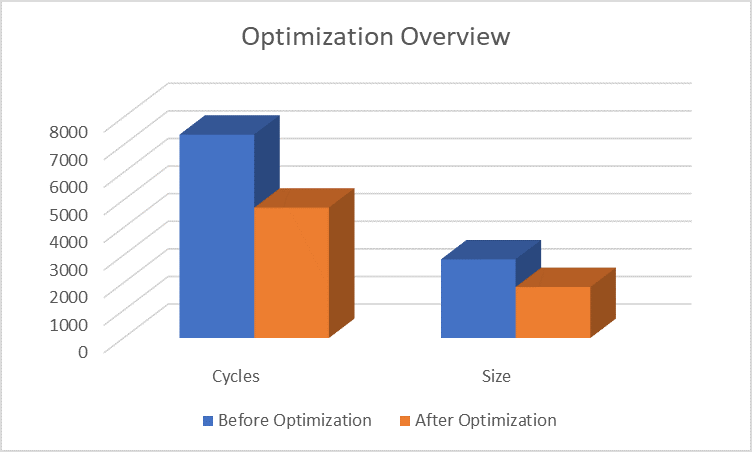
\includegraphics[width=0.8\linewidth]{image/quicksort_opt.png}
    \caption{对快排程序的优化结果}
\end{figure}

其中,程序的总体长度缩短了35.1\%,而在对于100个随机数的排序任务的执行过程中,总共执行的三地址代码数量减少了35.9\%,可见我们的优化在实际的程序中是卓有成效的。

\subsection{实验结果的一些细节}

\paragraph{DAG优化代码前后} 的效果如下图所示。

\begin{figure}[H]
    \centering
    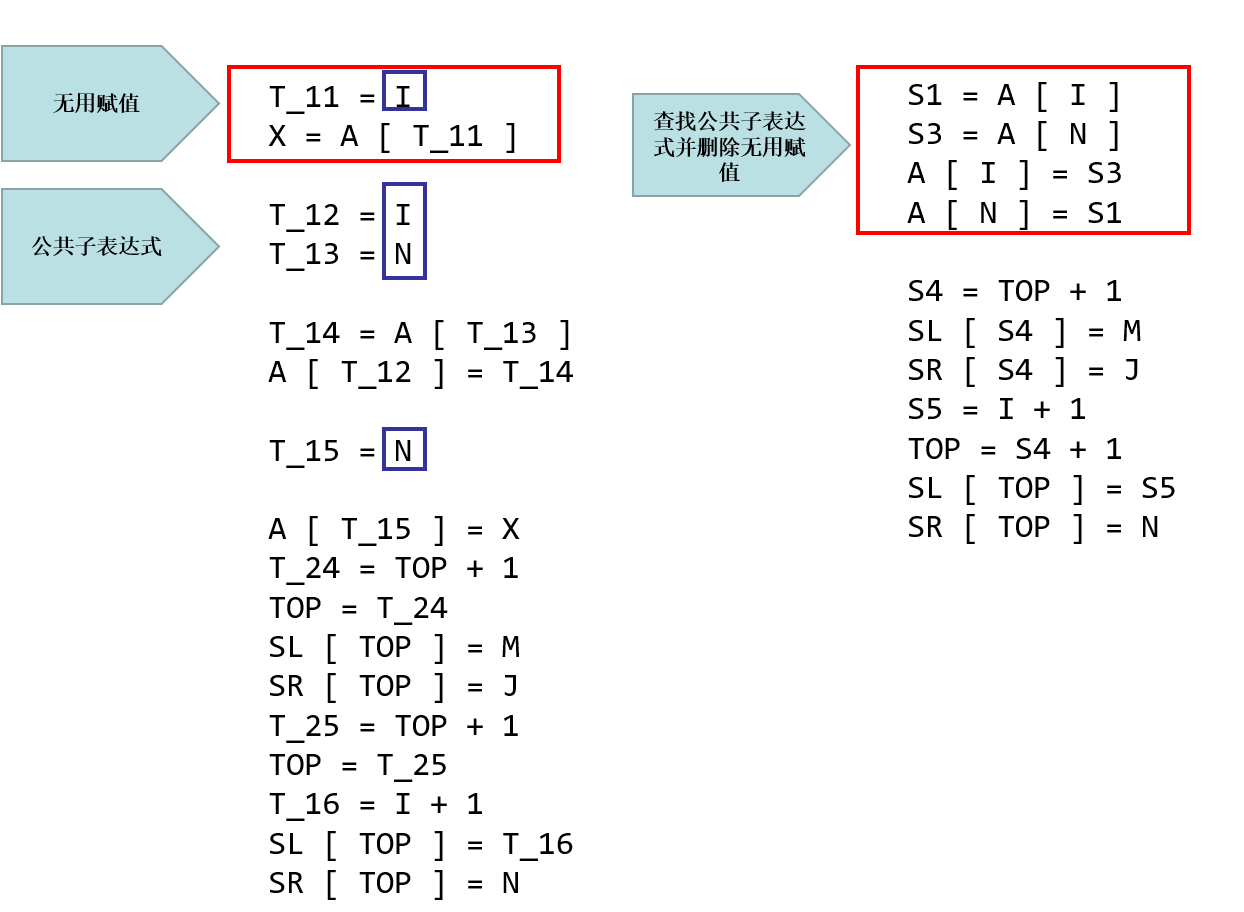
\includegraphics[width=0.8\linewidth]{image/res_dag.png}
    \caption{DAG优化代码前后对比}
\end{figure}

\paragraph{循环优化前后} 的效果如下图所示。

\begin{figure}[H]
    \centering
    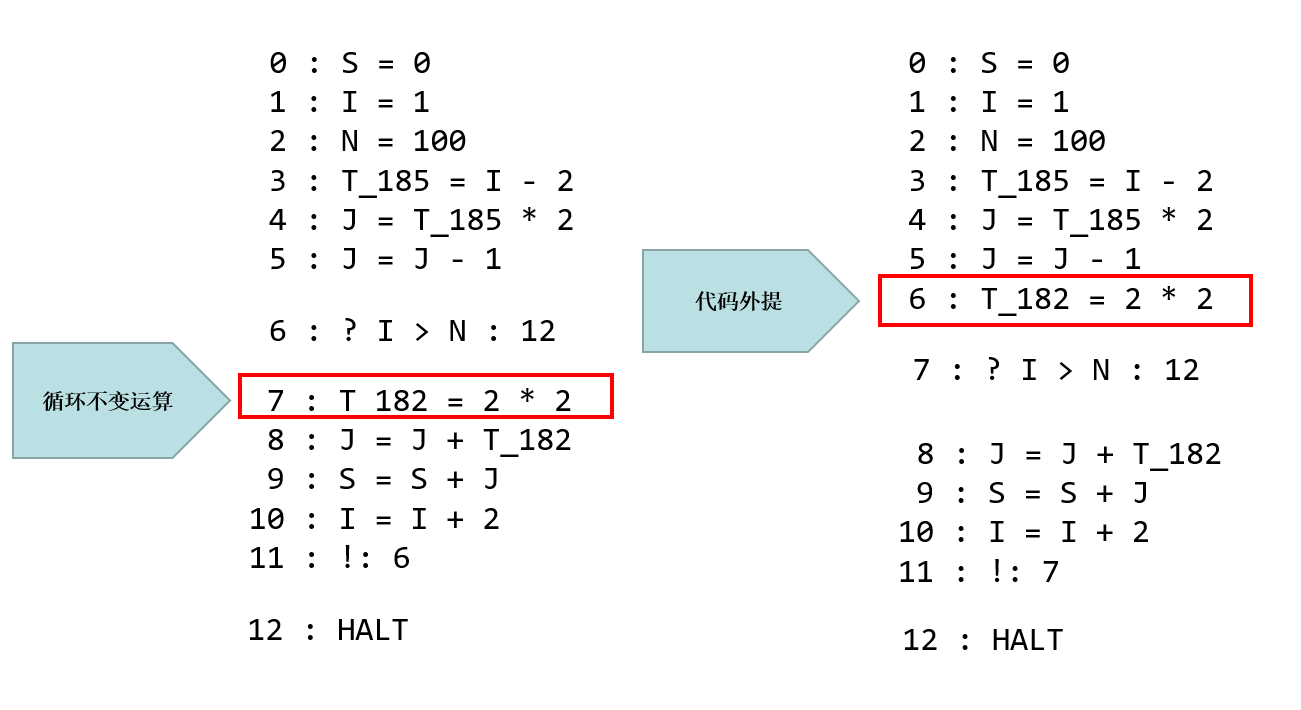
\includegraphics[width=0.8\linewidth]{image/res_loop.png}
    \caption{代码外提优化前后对比}
\end{figure}
\begin{figure}[H]
    \centering
    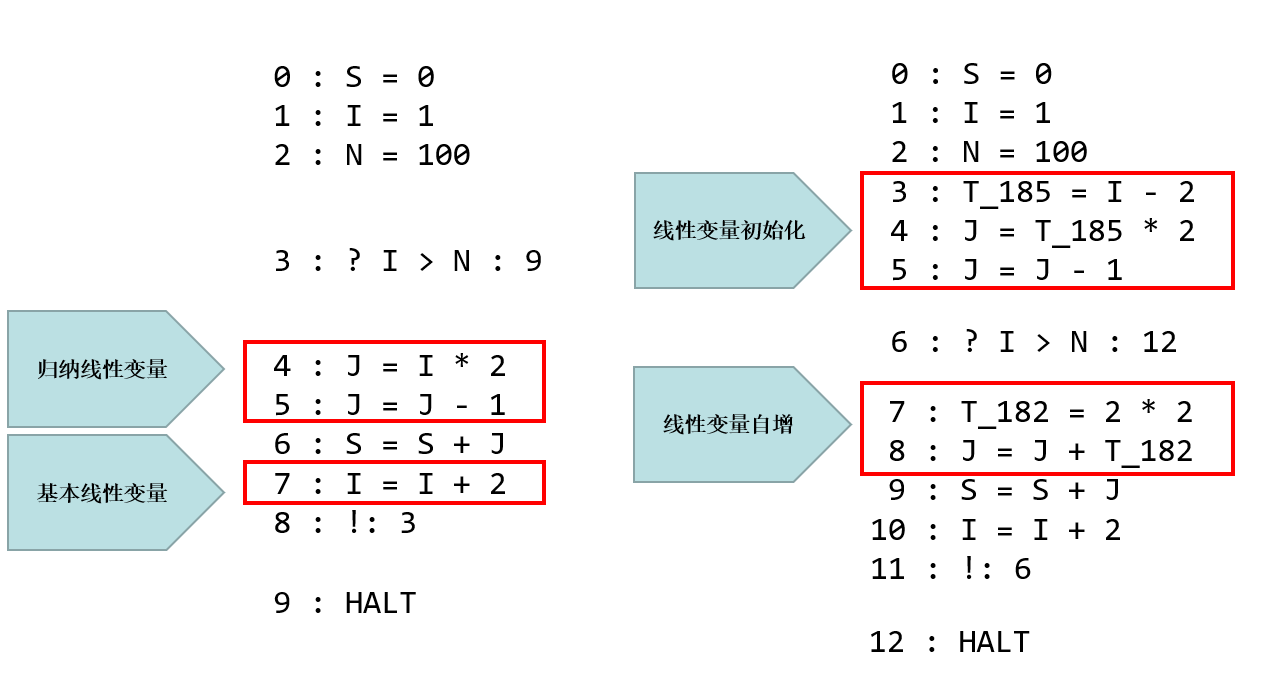
\includegraphics[width=0.8\linewidth]{image/res_for.png}
    \caption{强度削弱优化前后对比}
\end{figure}

\section{总结与思考}

\subsection{实验小结}

众所周知程序的性能是编程工作中非常重要的部分,尤其是高效率的数据结构和算法可以给程序运行带来很大的提升。但是除了在程序员考虑代码的时间空间复杂度层面的优化,其实在编译器层面,我们的所写的代码会被编译器执行一定的固定模式的优化,用来提升代码的效率,这就是我们所说的代码优化问题。

我们实现的功能有:虚拟机、图形化、切分基本块、自然循环的查找、活跃变量分析、基本块内优化、优化代码生成与死代码削除、循环不变量的查找及删除、代码外提、强度削弱。为保证程序的运行正确性,我们也有一些激进的优化没有实现。

在项目推进的过程中,课本编写的可参考的算法与代码都不多,优化的相关资料相比于其他模块的内容较少,对我们的自学能力与问题的思考解决能力都是很大的挑战。在编写的过程中我们每个模块遇见了不少问题,(局部优化以及循环优化),但是经过大家的讨论与共同思考,大部分问题最后都能够得到顺利解决。
通过此次大作业,我们对于编译过程中的代码优化过程有了一个深入的了解与学习,对整个编译过程的认知更上了一个台阶。


\subsection{实验亮点}

除了实验要求的内容外,我们认为,我们的实验还有如下亮点:
\begin{enumerate}
    \item 从头设计三地址代码的规范
    \item 运行三地址代码的虚拟机
    \item 图形化的展示界面
\end{enumerate}

\subsection{平台使用反馈}

平台使用感觉很不错,给的工具和界面都很好用,暂时没有什么建议。

\subsection{课程建议}

希望可以对大作业的指导文档可以更加准确更加详细。

\subsection{小组分工与成绩权重}

我们的项目通过GitHub平台进行开源,地址为;\url{https://github.com/42034301-5}。各成员的贡献和成绩权重如下。

\begin{itemize}
    \item 姜文渊:虚拟机、各项工具及规范、代码切分、代码生成、活跃变量及自然循环查找,20\% 。
    \item 杨鑫:循环不变量的查找、代码外提,20\%。
    \item 孟宇:基本块内优化、DAG图形界面,20\%。
    \item 李乐天:归纳变量的查找与删除、归纳变量的查找、DAG图形界面,20\%。
    \item 杨淳屹:算法总结归纳、文档编写20\%
\end{itemize}

\end{document}
